\documentclass{beamer}
\usepackage{etex}
\usetheme{Antibes}
\usepackage{amssymb,amsmath,amsthm}
\usepackage{graphicx}
\usepackage{caption}
\usepackage{subfig}
\newcommand{\bn}{\begin{enumerate}[i)]}
\newcommand{\en}{\end{enumerate}}
\newcommand{\im}{\item}
\newcommand{\CPT}[1]{\large{\textbf{CHAPTER #1}}}
\newcommand{\ir}[1]{\textbf{Remark #1}}
\newcommand{\ith}[1]{\textbf{Theorem #1}}
\newcommand{\idf}[1]{\textbf{Definition #1}}
\newcommand{\iex}[1]{\textbf{Example #1}}

%\definecolor{cardinal}{rgb}{0.77, 0.12, 0.23}
%\usecolortheme[named=cardinal]{structure}
%\setbeamercolor{block title}{bg=cardinal,fg=black}
 \usepackage{tikz}
 \usetikzlibrary{patterns,snakes,plotmarks}
 \usepackage{multirow}
% \usetikzlibrary{shadows}
\usepackage{epstopdf}
\usepackage{nicefrac}
\usepackage{lmodern}
\usepackage{pgfplots}
\usepackage{qtree}
\newcommand*{\Scale}[2][4]{\scalebox{#1}{\ensuremath{#2}}}%
\DeclareCaptionLabelSeparator{horse}{:\,\,} % change according to your needs
\captionsetup{
  labelsep = horse,
  figureposition = bottom % used to get the correct vertical space between the figure and the caption
}
\setbeamertemplate{caption}[numbered]
\setbeamertemplate{items}[circle]
\setbeamertemplate{enumerate items}[square]
\theoremstyle{definition}
\newtheorem*{exs}{Examples}
\newtheorem{ex}{Example}
\newtheorem*{exc}{Exercise}
%\usepackage{booktabs}
\setlength{\parindent}{0pt}
%\setbeameroption{show notes}
 \setbeamerfont{note page}{size=\tiny}
%\setbeamertemplate{note page}[plain]
%\setbeameroption{show only notes}
\title{Math 629 - Survival Analysis \\ Chapter 6: Extension
of the Cox Proportional Hazards Model for Time-Dependent Variables
}
\author{Drew Lazar}
\institute{Ball State University}
\date{\today}

\begin{document}
\begin{frame}
    \titlepage
\end{frame}



\section{Chapter 6}
\begin{frame}
\frametitle{Time-Dependent Covariates}
\begin{block}{Definitions of Time-Dependent Covariates}
\begin{itemize}
\item A time-dependent variable is defined as any variable whose value for a given subject may differ over time, $t$.
\item We distinguish three types of time-dependent variables:
\begin{enumerate}
\item \textbf{Defined:} These are typically products of time-dependent covariates and time-independent covariates used for testing PH assumption.
\item \textbf{Internal:} Variables such that the reason for the change in the value of variables depends on ``internal characteristics'' or behavior specific to subject.
\item \textbf{Ancillary:} Variables such that the value changes primarily because of ``external'' characteristics of the environment.
\end{enumerate}
\end{itemize}
\end{block}
\end{frame}

\begin{frame}
\frametitle{Time-Dependent Covariates}
\begin{block}{Examples of Time-Dependent Covariates}
\begin{itemize}
\item \textbf{Examples of Defined:} Race $\times$ time, E $\times \log(t-3)$ where $E$ is (0,1) exposure variable, E $\times g(t)$ where $g(t)$ is the Heaviside function.
\item \textbf{Examples of Internal:} Employment status at time $t$ if employment is based on performance, smoking status at time $t$, obesity level at time $t$.
\item \textbf{Examples of Ancillary:} Air pollution index at time $t$, employment status at time $t$ if employment is based on economic conditions.
\end{itemize}
\end{block}
\end{frame}

\begin{frame}
\frametitle{Time-Dependent Covariates}
\begin{block}{Examples of Time-Dependent Covariate}
\begin{itemize}
\item \textbf{Examples of part Internal, part Ancillary:} Heart transplant status at time $t$ (1 if received transplant, 0 if haven't at time $t$). Transplant status depends on internal characteristics:  age, other ailments, etc. and external characteristics: availability of donor, surgeon's schedule, etc.
\begin{columns}
    \begin{column}{0.48\textwidth}
        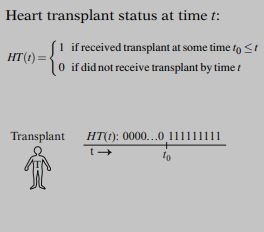
\includegraphics[width =\textwidth, height=4cm]{CH6_HT.JPG}
    \end{column}
    \hspace{-10pt}
    \begin{column}{0.48\textwidth}
         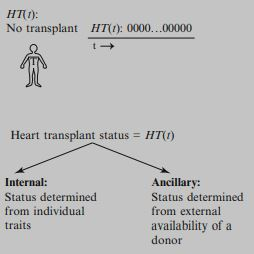
\includegraphics[width =\textwidth, height=4cm]{CH6_HTS2.JPG}
    \end{column}
\end{columns}
\end{itemize}
\end{block}
\end{frame}

\begin{frame}
\frametitle{The Extended Cox Model for Time-Dependent Variables}
\begin{block}{The Extended Cox Model for Time-Dependent Variables (cont'd)}
\[
h(t,X(t)) = h_0(t) \exp\left[\sum_{i=1}^{p_1} \beta_i X_i + \sum_{i=j}^{p_2} \delta_i X_i(t)\right]
\]
where
\[
X(t)=(X_1,\ldots,X_{p_1},X_j(t),\ldots,X_{p_2}(t))
\]
with $X_1,\ldots,X_{p_1}$ time-independent and $X_j(t),\ldots,X_{p_2}(t)$ time-dependent.
\end{block}
\end{frame}

\begin{frame}
\frametitle{The Extended Cox Model for Time-Dependent Variables}
\begin{block}{The Hazard Ratio Formula for the Extended Cox PH Model}
Let $X(t)$ and $X^*(t)$ be two specifications of the covariates $X(t)$. Then the HR with respect to this change in $X(t)$ is
\begin{align*}
HR(t) &= \frac{h(t,X^*(t))}{h(t,X(t))} \\
& = \exp\left[\sum_{i=1}^{p_1} \beta_i(X^*_i - X_i) + \sum_{i=j}^{p_2} \delta_i(X^*_i(t) - X_i(t))\right].
\end{align*}
As the $HR(t)$ depends on time, the extended Cox PH model does not satisfy the PH assumption.
\end{block}
\end{frame}


\begin{frame}
\frametitle{The Extended Cox Model for Time-Dependent Variables}
\begin{block}{Lag-time effect models}
You may want to account for the effect of a time-dependent covariate at previous periods. You can use a lag-time model:
\[
h(t,X(t)) = h_0(t) \exp\left[\sum_{i=1}^{p_1} \beta_i X_i + \sum_{i=j}^{p_2} \delta_i X_i(t-L_1)\right]
\]
where $L_1>0$.
An example of an lag-time effect model is
\[
h(t,EMP(t)) = h_0(t)\exp[\delta EMP(t-1)]
\]
where $EMP(t)$ is employment status at time $t$ in years and $EMP(t-1)$ is status at time $t-1$ (a year before time $t$).
\end{block}
\end{frame}

\begin{frame}
\frametitle{Assessing if Time-Independent Variables Satisfy the PH Assumption}
\begin{block}{Checking the PH assumption using defined time-dependent variables}
\begin{enumerate}
\item Assume we have $p$ time-dependent covariates $X=X_1,\ldots,X_p$.
\item To check the appropriateness of the Cox PH model
\begin{equation} \label{reducedCPH}
h(t,X) = h_0(t)\exp\left(\sum_{i=1}^p \beta_i X_i \right)
\end{equation}
We introduce defined time-dependent covariates in an extended Cox PH model
\begin{equation} \label{fullintCPH}
h(t,X(t)) = h_0(t) \exp\left[\sum_{i=1}^p \beta_i X_i + \sum_{i=1}^p \delta_i X_i g_i(t)\right]
\end{equation}
\end{enumerate}
\end{block}
\end{frame}


\begin{frame}
\frametitle{Assessing if Time-Independent Variables Satisfy the PH Assumption}
\begin{block}{Checking the PH assumption using defined time-dependent variables}
\begin{itemize}
\item An overall test of interaction between time and our covariates
\[
H_0: \delta_i = 0 \text{ for all } i \text{ vs. } \delta_i \neq 0 \text{ for some } i.
\]
\item Our full model is \eqref{fullintCPH} and our reduced model is \eqref{reducedCPH}. Our test statistic and its distribution is:
\vspace{-10pt}
\[
-2(\ln(L_R) - \ln(L_F)) \sim \chi^2(p)
\]
\item A test of covariate $X_k$ ``one-at-a-time" uses reduced model
\vspace{-10pt}
\[
h(t,X(t)) = \exp\left[\sum_{i=1}^p \beta_i X_i + \delta_k X_k g_k(t)\right]
\]
\end{itemize}
\end{block}
\end{frame}

\begin{frame}
\frametitle{Modeling and testing interaction of time-independent variables with time.}
\begin{block}{Functions used for assessing interaction}
\begin{itemize}
\item You want to choose a function, $g_i(t)$, that reflects the possible interaction between the covariate $X_i$ and time.
\item For example, assume the study is over the period (1,6). If the effect of an exposure variable $E (0 \text{ or } 1)$ is
\begin{enumerate}
\item increasing but decelerating with time you might use $g_i(t)= \ln(t)$.
\item decreasing rapidly with time you might use $g_i(t)=\exp(-(t-1))$.
\item increasing rapidly with time you might use $g_i(t)=(t-1)^2+2$ where 2 reflects the hazard ratio at the start of the study.
\end{enumerate}
\end{itemize}
\end{block}
\end{frame}


\begin{frame}
\frametitle{Modeling and testing interaction of time-independent variables with time.}
\begin{block}{Functions used for assessing interaction (cont'd)}
\begin{enumerate}
\item Often the PH assumption is met with different ratios for different intervals in the study.
\item For example, before time $t_0$ women have twice the hazard as men and after time $t_0$ they have 1/2 the hazard.
\item In this case you can partition the data by time or you can use an extended Cox PH model with a heaviside function.
\end{enumerate}
\end{block}
\end{frame}


\begin{frame}
\frametitle{Modeling and testing interaction of time-independent variables with time.}
\begin{block}{Functions used for assessing interaction (cont'd): using the Heaviside function}
\begin{columns}
    \begin{column}{0.48\textwidth}
        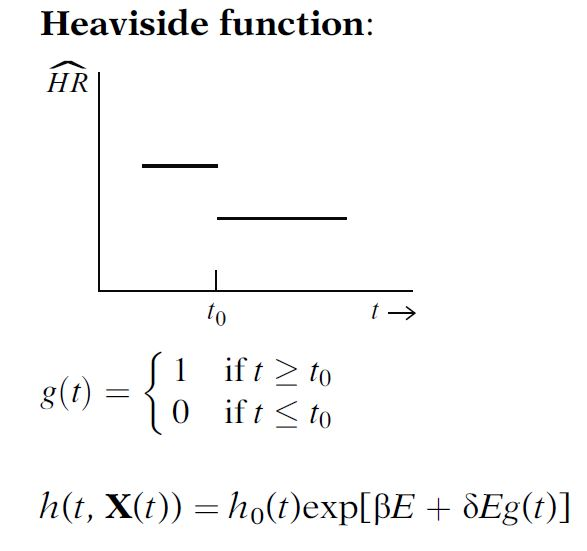
\includegraphics[width =\textwidth, height=4cm]{CH6_HeSi.JPG}
    \end{column}
    \hspace{-10pt}
    \begin{column}{0.48\textwidth}
         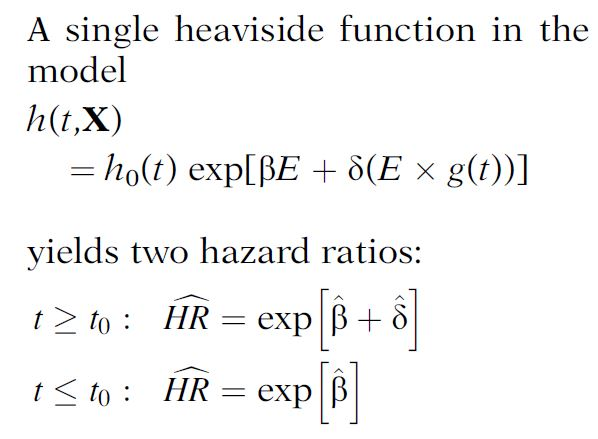
\includegraphics[width =\textwidth, height=4cm]{CH6_HeSi2.JPG}
    \end{column}
\end{columns}
\end{block}
\end{frame}

\begin{frame}
\frametitle{Modeling and testing interaction of time-independent variables with time.}
\begin{block}{Functions used for assessing interaction (cont'd): using the Heaviside function}
\vspace{-20pt}
\begin{center}
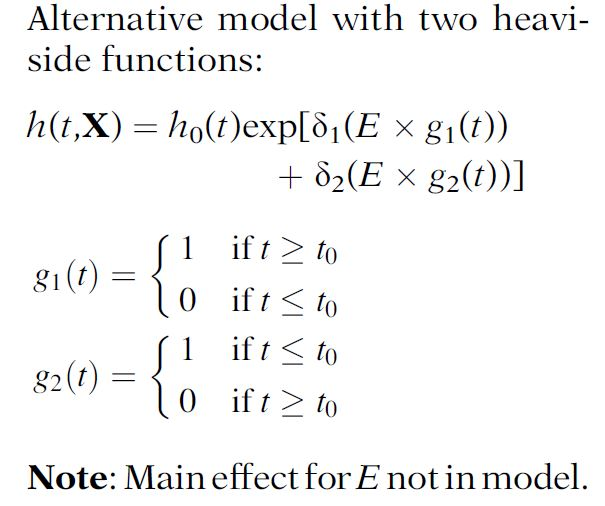
\includegraphics[width =\textwidth, height=5.2cm]{CH6_HeSi3.JPG}
\end{center}
\end{block}
\end{frame}

\begin{frame}
\frametitle{Modeling and testing interaction of time-independent variables with time.}
\begin{block}{Problem 6.1 - Functions used for assessing interaction (cont'd): using the Heaviside function}
Assume for a our survival data we have a single exposure variable, $E$. We believe that in each of the intervals of the study
\[
(0,.5], (0.5,1], (1,1.5], [1.5,\infty)
\]
the HR of $E$ is constant but different. Create an extended Cox PH to model this situation.
\end{block}
\end{frame}

\begin{frame}
\frametitle{Modeling and testing interaction of time-independent variables with time.}
\begin{block}{Problem 6.1 - Functions used for assessing interaction (cont'd): using the Heaviside function}
\begin{columns}
    \begin{column}{0.48\textwidth}
        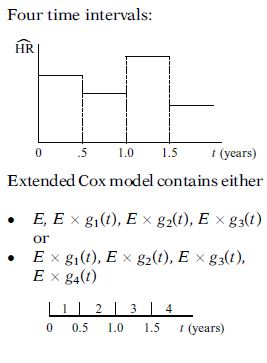
\includegraphics[width =\textwidth, height=5cm]{CH6_fhev.JPG}
    \end{column}
    \hspace{-10pt}
    \begin{column}{0.48\textwidth}
         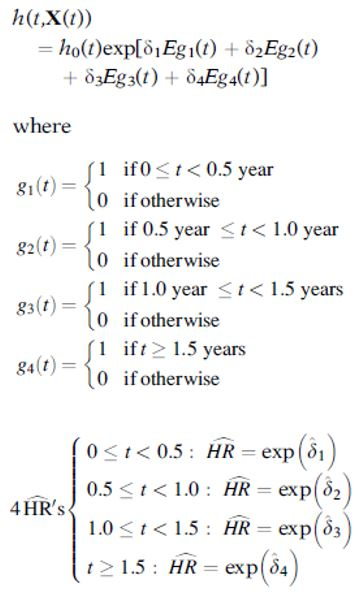
\includegraphics[width =\textwidth, height=5cm]{CH6_fhev2.JPG}
    \end{column}
\end{columns}
\end{block}
\end{frame}

\begin{frame}
\frametitle{Modeling and testing interaction of time-independent variables with time.}
\begin{block}{Problem 6.2 - An Application of the Extended Cox Model to An Epidemiologic Study on Heroin
Addiction}
A 1991 Australian study by Caplehorn et al., compared retention in two methadone treatment clinics for heroin addicts. A patient’s survival time (T) was determined as the time in days until the patient dropped out of the clinic or was censored at the end of the study clinic.
\vspace{-10pt}
\begin{center}
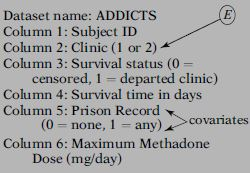
\includegraphics[height=3.2cm]{CH6_Heroin1.JPG}
\end{center}
\end{block}
\end{frame}

\begin{frame}
\frametitle{Modeling and testing interaction of time-independent variables with time.}
\begin{block}{Problem 6.2 - An Application of the Extended Cox Model to An Epidemiologic Study on Heroin Addiction (cont'd)}
\begin{enumerate}
\item For the variables Clinic, Prison and Dose test the PH assumption through a GOF test using Shoenfeld residuals.
\item For the variable that doesn't satisfy the PH assumption according to your GOF test, create adjusted survival curves with the other variables in the model.
\item Based on 2) create an extended Cox PH model to estimate the effect of the variable that doesn't satisfy the Cox PH model. Estimate the HR of this variable with time.
\item Create another extended Cox PH as an alternative to 3) above. Estimate the HR of this variable with time based on this model.
\end{enumerate}
\end{block}
\end{frame}

\begin{frame}
\frametitle{Modeling and testing interaction of time-independent variables with time.}
\begin{block}{Problem 6.2 - An Application of the Extended Cox Model to An Epidemiologic Study on Heroin Addiction (cont'd)}
\begin{columns}
    \begin{column}{0.48\textwidth}
        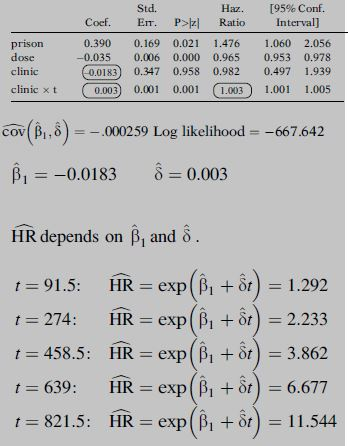
\includegraphics[width =\textwidth, height=5cm]{CH6_P2.JPG}
    \end{column}
    \hspace{-10pt}
    \begin{column}{0.48\textwidth}
         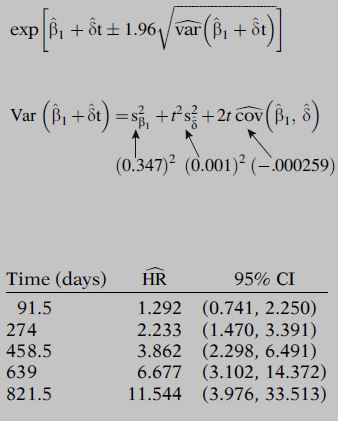
\includegraphics[width =\textwidth, height=5cm]{CH6_P2a.JPG}
    \end{column}
\end{columns}
\end{block}
\end{frame}


\begin{frame}
\frametitle{Modeling and testing interaction of time-independent variables with time.}
\begin{block}{Example 6.1 - An Application of the Extended Cox Model to the Analysis of the Stanford Heart Transplant Data}
In the 1977 Stanford Heart Transplant
Study, patients identified as being eligible for a
heart transplant were followed until death or
censorship. Sixty-five of these patients received
transplants at some point during follow-up,
whereas thirty-eight patients did not receive a
transplant. There were, thus, a total of $n = 103$
patients. The goal of the study was to assess
whether patients receiving transplants survived
longer than patients not receiving transplants.
\end{block}
\end{frame}


\begin{frame}
\frametitle{Modeling and testing interaction of time-independent variables with time.}
\begin{block}{Example 6.1 - An Application of the Extended Cox Model to the Analysis of the Stanford Heart Transplant Data}
There are three internal time-dependent covariates in this data set.
\vspace{-15pt}
\begin{enumerate}
\item The exposure variable: heart transplant status, $H(t)$, at $t$.
\item The covariates: tissue mismatch score at the time of transplant, $TMS(t)$ and age at time of transplant, $AGE(t)$.
\end{enumerate}
\begin{center}
 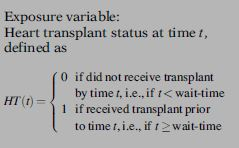
\includegraphics[width = 5cm, height=3cm]{CH6_tnsp1.JPG}
 \end{center}
\end{block}
\end{frame}

\begin{frame}
\frametitle{Modeling and testing interaction of time-independent variables with time.}
\begin{block}{Example 6.1 - An Application of the Extended Cox Model to An Epidemiologic Study on the Treatment of Heroin Addiction}
\begin{columns}
    \begin{column}{0.48\textwidth}
        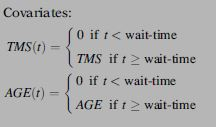
\includegraphics[width =\textwidth, height=3cm]{CH6_transp2.JPG}
    \end{column}
    \hspace{-10pt}
    \begin{column}{0.48\textwidth}
         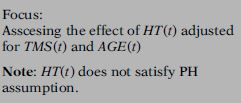
\includegraphics[width =\textwidth, height=4cm]{CH6_transp3.JPG}
    \end{column}
\end{columns}
\end{block}
\end{frame}

\begin{frame}
\frametitle{Modeling and testing interaction of time-independent variables with time.}
\begin{block}{Example 6.1 - An Application of the Extended Cox Model to the Analysis of the Stanford Heart Transplant Data}
Our model is:
\[
h(t,X(t))= h_0(t) \exp[\delta_1 HT(t) + \delta_2 TMS(t) + \delta_3 AGE(t)]
\]
And the results of fitting the model are:
\begin{center}
 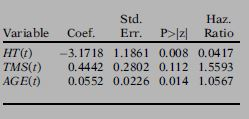
\includegraphics[width = 5cm, height=3cm]{CH6_trnsp4}
 \end{center}
\end{block}
\end{frame}

\begin{frame}
\frametitle{Modeling and testing interaction of time-independent variables with time.}
\begin{block}{Example 6.1 - An Application of the Extended Cox Model to the Analysis of the Stanford Heart Transplant Data}
With our model we can estimate at:
\begin{enumerate}
\item any particular time of transplant, $t$
\item  for any particular TMS score at $t$, and
\item for any particular Age at $t$
\end{enumerate}
the hazard ratio of receiving the transplant at time $t$:
\[
\hat{HR}(t) = \exp[\hat{\delta}_1 + \hat{\delta}_2 TMS(t) + \hat{\delta}_3 AGE(t)]
\]
\end{block}
\end{frame}

\begin{frame}
\frametitle{Modeling and testing interaction of time-independent variables with time.}
\begin{block}{Example 6.1 - An Application of the Extended Cox Model to the Analysis of the Stanford Heart Transplant Data}
    \begin{center}
        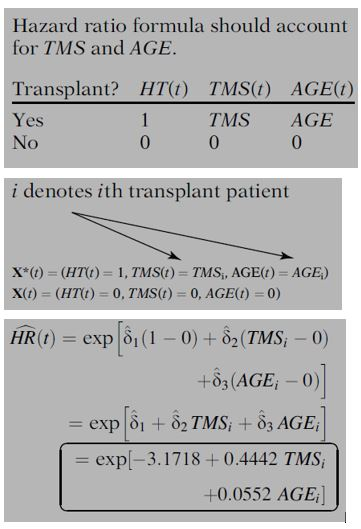
\includegraphics[width =5cm, height=5.5cm]{CH6_trnsp5.JPG}
    \end{center}
\end{block}
\end{frame}

\begin{frame}
\begin{block}{Example 6.1 - An Application of the Extended Cox Model to An Epidemiologic Study on the Treatment of Heroin Addiction}
The range of the covariates must be as in the data: The TMS range must be: $(0-3.05)$ and the Age range: $(12-64)$.
\begin{itemize}
\item The hazard ratio of someone with age of 30 and TMS of .5 is
\[ \exp[-.31718 + 0.4442\times 0.5 + .0552 \times 30] = 0.2768997
\]
\item The hazard ratio of someone with age of 50 and TMS of 2 is
\[ \exp[-.31718 + 0.4442\times 2 + .0552 \times 50] = 1.636566
\]
\end{itemize}
\end{block}
\end{frame}

\begin{frame}
\frametitle{Maximum Likelihood Estimation with time dependent covariates}
\begin{block}{Example 6.2 - Partial MLE of the Extended Cox PH Model}
Consider the survival data about Bary, Gary, Susan and John.
\begin{center}
\begin{tabular}{ c c c c } \hline
 Name & Time & Status & Coupon \\ \hline
Barry & 2 & 1 & 1 \\
 Gary & 3 & 0 & 1 \\
Susan & 5 & 1 & 0 \\
  John & 8 & 1 & 1 \\
\end{tabular}
\end{center}
\end{block}
We want to model the interaction of Coupon with time $g(t)=t$. That is, we want to estimate $\beta$ and $\delta$ in
\[
h(t,X) = h_0(t) \exp[\beta X+ \delta X *t]
\]
where $X=\text{Coupon}$.
\end{frame}

\begin{frame}
\frametitle{ML Estimation with time dependent covariates}
\begin{block}{The data in counting process format}
\begin{table}[]
\begin{tabular}{c c c c c c}
Name  & Start & Time & Status & Coupon & Coupon $\times$ Time \\ \hline
Barry & 0     & 2    & 1      & 1      & 2                    \\
Gary  & 0     & 2    & 0      & 1      & 2                    \\
Gary  & 2     & 3    & 0      & 1      & 3                    \\
Susan & 0     & 2    & 0      & 0      & 0                    \\
Susan & 2     & 5    & 1      & 0      & 0                    \\
John  & 0     & 2    & 0      & 1      & 2                    \\
John  & 2     & 5    & 0      & 1      & 5                    \\
John  & 5     & 8    & 1      & 1      & 8
\end{tabular}
\end{table}
\end{block}
\end{frame}

\begin{frame}
\frametitle{ML Estimation with time dependent covariates}
\begin{block}{Our (extended) partial likelihood, $L$}
\begin{align*}
L_1 & = \frac{e^{\beta+2\delta}}{e^{\beta+2\delta} + e^{\beta+2\delta} + 1 + e^{\beta+2\delta}} \\
L_2 & = \frac{1}{1+e^{\beta+5\delta}} \\
L_3 & = \frac{e^{\beta + 8\delta}}{e^{\beta + 8\delta}} \\
L & = L_1 \times L_2 \times L_3
\end{align*}
\end{block}
\end{frame}
\end{document}






